\documentclass[12pt,a4paper]{article}
\usepackage{fontspec}
\usepackage{polyglossia}
\setdefaultlanguage{russian}
\setotherlanguage{english}
\setmainfont{STIX Two Text}
\setmonofont{Menlo}
\newfontfamily\cyrillicfonttt{Menlo}
\usepackage[a4paper,margin=2cm]{geometry}
\usepackage{graphicx}
\graphicspath{{report-assets/lab3/}}
\usepackage{longtable,tabularx,array,booktabs}
\usepackage{float}
\usepackage{caption}
\usepackage{enumitem}
\usepackage{pdflscape}
\usepackage{xurl}
\usepackage{tikz}
\usetikzlibrary{arrows.meta,positioning,fit,backgrounds,shapes.geometric}
\usepackage{hyperref}
\hypersetup{colorlinks=true,linkcolor=blue,urlcolor=blue}
\setlength{\parindent}{1.25cm}
\setlength{\parskip}{0.25em}
\renewcommand{\arraystretch}{1.18}
\setlist{nosep,leftmargin=1.5em}
\sloppy

\setcounter{tocdepth}{2}

\begin{document}
\begin{titlepage}
\centering
{\large Университетская лабораторная работа\par}
\vspace{2.5cm}
{\LARGE\bfseries Отчет по лабораторной работе № 3\par}
\vspace{0.6cm}
{\Large Разработка модели угроз и модели нарушителя программной системы\par}
\vspace{1.8cm}
\begin{tabular}{p{4cm}p{11cm}}
Дисциплина: & Основы разработки защищенного программного обеспечения и компьютерных сетей\\
Вариант: & 19 — Система учета транспортных средств организации\\
Исходная версия: & v0.2\\
Версия ЛР: & v0.3\\
Студент: & Мостовая Полина Андреевна\\
Группа: & ИУСбд-02-23
\end{tabular}
\vfill
{\large 2026\par}
\end{titlepage}
\tableofcontents
\clearpage

\section{Цель работы}
Цель работы — освоить выявление угроз программной системе, описание возможностей и ограничений нарушителей, построение диаграммы потоков данных, предварительную оценку рисков и обоснование защитных мер. Модель связывается с конкретными функциями и активами системы учета транспорта.

\section{Исходное состояние и предметная область}
Сквозной проект — система учета транспортных средств организации. Она предназначена для ведения реестра автопарка, закрепления транспорта за водителями, планирования поездок, учета пробега и контроля технического состояния.

Исходный лабораторный тег \texttt{v0.2} указывает на commit \texttt{4026dd7}. Документация предыдущего этапа включает активы AS-1–AS-10, роли и предварительную матрицу доступа, требования SEC-1–SEC-13 и приемочные сценарии AT-1–AT-6.

Фактически приложение загружает настройки из переменных окружения и файла \texttt{.env}, проверяет имя приложения, режим работы и минимальную длину \texttt{APP\_SECRET\_KEY}, затем печатает стартовое сообщение без значения секрета. Сетевого интерфейса, аутентификации и авторизации, базы данных, учета транспортных средств и поездок и журнала аудита нет. Тестовый набор содержит три теста стартового сообщения.

Проектируемое состояние включает пользовательский интерфейс, процессы аутентификации и учета, базу данных учетных записей и транспортных данных, отчетность и журналирование. Эти компоненты помечены как запланированные. Сценарий угрозы не доказывает наличие уязвимости, а требование не доказывает, что контроль уже работает.

\begin{figure}[H]
\centering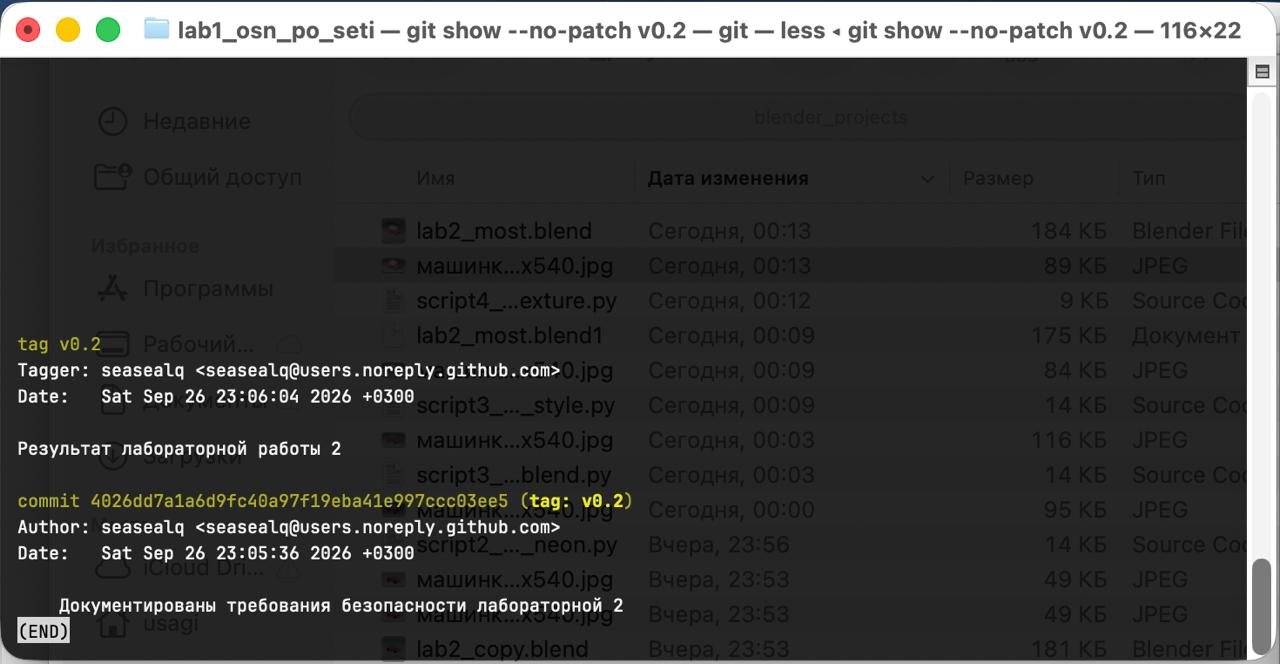
\includegraphics[width=0.94\textwidth]{01-v02-tag.jpg}
\caption{Просмотр исходной метки v0.2 и commit.}
\end{figure}
\begin{figure}[H]
\centering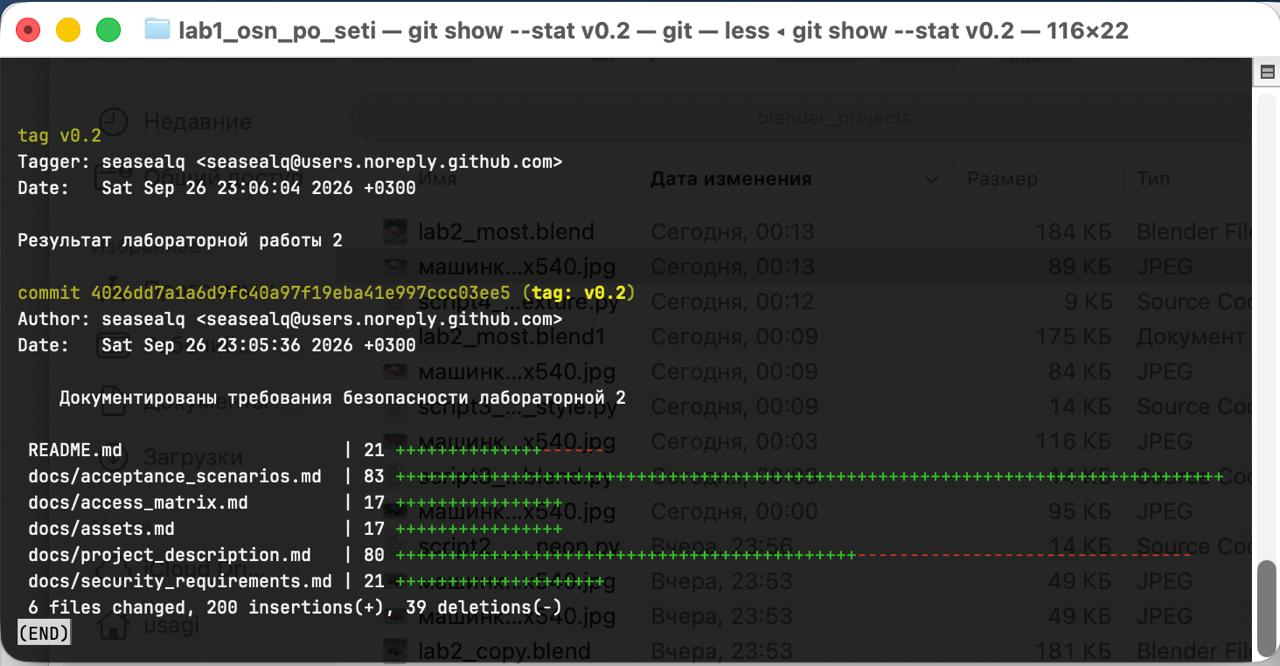
\includegraphics[width=0.94\textwidth]{02-v02-documentation.jpg}
\caption{Состав документации лабораторной работы № 2.}
\end{figure}

\section{Область анализа, допущения и ограничения}
Рассматриваются вход, просмотр и ведение карточек ТС, назначения, поездки, отчеты, техническое состояние, управление доступом и аудит. Внешняя кадровая система, бухгалтерия, телематика, фактическое местоположение и физическое управление транспортом исключены. Для учебных проверок используются искусственные данные.

\begin{longtable}{p{1.2cm}p{5.0cm}p{5.3cm}p{3.0cm}}
\caption{Допущения модели}\\
\toprule ID & Допущение & Если оно неверно & Статус защиты\\\midrule\endfirsthead
\toprule ID & Допущение & Если оно неверно & Статус защиты\\\midrule\endhead
ASM-01 & Клиент обращается к приложению; прямой доступ рабочего места к БД не предоставляется & Нужен отдельный анализ сетевого доступа к СУБД & Требует проверки; интерфейса нет\\
ASM-02 & Клиентские запросы и переданные идентификаторы недоверенные & Возрастет риск подмены владельца или назначения & Серверная проверка запланирована\\
ASM-03 & Учетная запись приложения к БД имеет только необходимые права & Компрометация процесса затронет больше данных & Требует проверки после выбора СУБД\\
ASM-04 & Учебная среда использует искусственные данные & Реальные данные требуют пересмотра последствий и доступа & Искусственные примеры применяются; эксплуатация не подтверждена\\
ASM-05 & Журнал логически отделен от учетных данных, доступ ограничен & Изменение данных может скрыть историю действий & Требует проверки; физическое разделение не определено\\
ASM-06 & Изменения назначения, состояния ТС и ролей связаны с субъектом и результатом & Сложнее расследовать фиктивную выдачу/возврат и смену ролей & Требование сформулировано; механизм не реализован\\
\bottomrule
\end{longtable}

Модель является проектным анализом, а не тестом на проникновение. Компрометация ОС, физическая безопасность автомобилей и правовые режимы реальных персональных данных не исследуются.

\section{Модель нарушителя}
\begin{longtable}{p{1.1cm}p{3.2cm}p{4.3cm}p{5.8cm}}
\caption{Типы нарушителей и ограничения}\\
\toprule ID & Тип, исходный доступ & Возможности и цель & Отсутствующие права и ограничения\\\midrule\endfirsthead
\toprule ID & Тип, исходный доступ & Возможности и цель & Отсутствующие права и ограничения\\\midrule\endhead
N-01 & Внешнее лицо без учетной записи; публичного интерфейса сейчас нет & Может посылать запросы к будущей форме входа; цель — получить учетный доступ или нарушить доступность & Нет учетной записи, сервера и БД; планируются аутентификация, лимиты и запрет прямого доступа к БД\\
N-02 & Водитель с собственной учетной записью, если вход реализован & Меняет параметры своих запросов; может попытаться прочитать чужую поездку или подменить отчет & Нет прав диспетчера, администратора и ОС; серверная проверка записи запланирована\\
N-03 & Диспетчер с прикладной учетной записью & Ведет карточки автопарка и назначения; может неправомерно изменить учетную историю & Не управляет ролями, ОС или СУБД; разделение полномочий и аудит проектируются\\
N-04 & Администратор безопасности приложения & Управляет учетными записями и ролями; может пытаться скрыть действие & Нет автоматических прав ОС/БД; нужны аудит и ограничение прикладных полномочий\\
N-05 & Администратор среды выполнения (ОС) & Имеет локальный доступ к файлам и процессу в пределах ОС & Не является автоматически администратором приложения или СУБД; разделение системных учетных записей запланировано\\
\bottomrule
\end{longtable}
Администратор приложения и администратор ОС рассматриваются отдельно: у них разные полномочия и границы доступа.

\section{Диаграмма потоков данных}
Диаграмма показывает логические потоки проектируемой системы, а не физическую схему сети. Для читаемости на ней показаны основные направления; потоки F1–F17 описаны после рисунка.

\begin{landscape}
\begin{figure}[H]
\centering
\resizebox{24cm}{!}{%
\begin{tikzpicture}[
  ext/.style={draw,rounded corners,fill=blue!7,align=center,text width=3.5cm,minimum height=1cm,font=\small},
  proc/.style={draw,ellipse,fill=green!8,align=center,text width=3.4cm,minimum height=1.2cm,font=\small},
  data/.style={draw,cylinder,shape border rotate=90,aspect=0.25,fill=orange!12,align=center,text width=3cm,minimum height=1.1cm,font=\small},
  flow/.style={-{Stealth[length=2.2mm]},thick},
  flowboth/.style={{Stealth[length=2.2mm]}-{Stealth[length=2.2mm]},thick},
  every node/.style={font=\small}]
\node[ext] (E1) at (0,3) {E1\\Сотрудник\\(водитель, диспетчер, руководитель)};
\node[ext] (E2) at (0,0) {E2\\Администратор безопасности приложения};
\node[ext] (E3) at (0,-3) {E3\\Администратор среды выполнения};
\node[proc] (P1) at (5,3) {P1\\Аутентификация и обработка запросов};
\node[proc] (P2) at (10,3) {P2\\Учет автопарка и поездок};
\node[proc] (P3) at (15,3) {P3\\Формирование отчетов};
\node[data] (D1) at (7.5,-0.5) {D1\\База данных учета};
\node[proc] (P4) at (10,-3.3) {P4\\Регистрация событий безопасности};
\node[data] (D2) at (15,-3.3) {D2\\Журнал событий безопасности};

\draw[flowboth] (E1.east) to[out=5,in=175] node[above,fill=white,inner sep=1pt]{F1/F2} (P1.west);
\draw[flowboth] (E2.east) to[out=10,in=225] node[above,sloped,fill=white,inner sep=1pt]{F3/F4} (P1.south west);
\draw[flow] (P1.east) -- node[above,fill=white,inner sep=1pt]{F5} (P2.west);
\draw[flow] (P2.north) -- ++(0,1.8) -| node[pos=0.25,above,fill=white,inner sep=1pt]{F6} (E1.north);
\draw[flow] (P2.east) -- node[above,fill=white,inner sep=1pt]{F7} (P3.west);
\draw[flow] (P3.north) -- ++(0,2.6) -| node[pos=0.25,above,fill=white,inner sep=1pt]{F8} (E1.north);
\draw[flowboth] (P2.south west) to[bend right=8] node[pos=0.55,right,fill=white,inner sep=1pt]{F9/F10} (D1.north east);
\draw[flowboth] (P1.south east) to[bend left=8] node[pos=0.55,left,fill=white,inner sep=1pt]{F11/F12} (D1.north west);
\draw[flow] (P1.south west) -- ++(-0.5,-0.7) |- node[pos=0.8,below,fill=white,inner sep=1pt]{F13} (P4.west);
\draw[flow] (P2.south) -- node[right,fill=white,inner sep=1pt]{F14} (P4.north);
\draw[flowboth] (P4.east) to[bend left=10] node[above,fill=white,inner sep=1pt]{F15/F16} (D2.west);
\draw[flow] (E3.east) to[out=0,in=250] node[below,sloped,fill=white,inner sep=1pt]{F17} (P1.south west);

\node[draw,dashed,rounded corners,fit=(P1)(P2)(P3)(D1)(P4)(D2),inner sep=12pt,label=above:{TB-01: граница клиента и приложения}] {};
\node[draw,dashed,rounded corners,fit=(D1),inner sep=8pt,label={[fill=white]above:{TB-02}}] {};
\node[draw,dashed,rounded corners,fit=(D2),inner sep=8pt,label=right:{TB-03}] {};
\end{tikzpicture}%
}
\caption{DFD проектируемой системы учета транспортных средств.}
\end{figure}
\end{landscape}

\begin{longtable}{p{1.5cm}p{13.0cm}}
\caption{Элементы и потоки DFD}\\
\toprule ID & Описание и статус\\\midrule\endfirsthead
\toprule ID & Описание и статус\\\midrule\endhead
E1 & Сотрудник: водитель, диспетчер или руководитель; проектируемая внешняя сущность.\\
E2 & Администратор безопасности приложения; проектируемая внешняя сущность.\\
E3 & Администратор среды выполнения; локальная загрузка конфигурации существует, серверные полномочия не определены.\\
P1 & Аутентификация и обработка запросов; проектируется.\\
P2 & Учет карточек ТС, назначений, поездок и технического состояния; проектируется.\\
P3 & Формирование отчетов; проектируется.\\
P4 & Регистрация событий аудита; проектируется.\\
D1 & База профилей, ролей, карточек, поездок и состояния; проектируется.\\
D2 & Логическое хранилище событий безопасности; проектируется, физическое разделение не подтверждено.\\
F1 & Учетные данные и пользовательский запрос от E1 к P1; проектируется.\\
F2 & Результат входа или разрешенный ответ от P1 к E1; проектируется.\\
F3 & Команда управления пользователем/ролью от E2 к P1; проектируется.\\
F4 & Результат административной операции от P1 к E2; проектируется.\\
F5 & Разрешенный запрос учетной функции от P1 к P2; проектируется.\\
F6 & Карточка ТС, назначение, поездка или состояние от P2 к E1; проектируется.\\
F7 & Подготовленные данные учета от P2 к P3; проектируется.\\
F8 & Агрегированный отчет от P3 к E1; проектируется.\\
F9 & Чтение/запись учетных данных от P2 к D1; проектируется.\\
F10 & Найденные записи от D1 к P2; проектируется.\\
F11 & Учетные данные и роли от P1 к D1; проектируется.\\
F12 & Результат проверки учетной записи от D1 к P1; проектируется.\\
F13 & Событие входа/отказа от P1 к P4; проектируется.\\
F14 & Событие изменения учета от P2 к P4; проектируется.\\
F15 & Запись аудита от P4 к D2; проектируется.\\
F16 & События для разрешенного просмотра от D2 к P4; проектируется.\\
F17 & Конфигурация от E3 к P1; локальная загрузка реализована, серверная связь проектируется.\\
\bottomrule
\end{longtable}

\subsection{Границы доверия}
\begin{itemize}[leftmargin=1.2cm]
\item \textbf{TB-01 — клиент/приложение.} F1–F6 и F8. Проверяются подлинность пользователя, роль, право на конкретный объект, формат и размер полей, минимизация ответа.
\item \textbf{TB-02 — приложение/БД.} F9–F12. Проверяются минимальные права учетной записи БД, безопасные параметризованные запросы и запрет прямого доступа клиентов.
\item \textbf{TB-03 — приложение/аудит.} F13–F16. Проверяются источник и формат события, права чтения/изменения, объем хранения и реакция на заполнение.
\end{itemize}
Граница доверия может находиться между процессами или учетными записями одного сервера: она определяется полномочиями и проверками, а не только сетевой топологией.

\subsection{Точки входа}
\begin{longtable}{p{3.3cm}p{4.2cm}p{6.5cm}}
\caption{Точки входа проектируемой системы}\\
\toprule Точка & Данные и источник & Проверки и состояние\\\midrule\endfirsthead
\toprule Точка & Данные и источник & Проверки и состояние\\\midrule\endhead
Форма входа & Идентификатор и пароль; N-01/сотрудник & Проверка учетной записи, ограничение попыток, безопасный ответ; проектируется.\\
Чтение карточки/поездки & ID записи; водитель/диспетчер & Право на конкретную запись и минимизация ответа; проектируется.\\
Изменение карточки ТС & Поля и статус; диспетчер & Формат, допустимые поля/переходы и роль; проектируется.\\
Назначение, выдача/возврат & ID ТС, водителя, поездки, даты & Существование объектов, отсутствие конфликта, история; проектируется.\\
Отчет о поездке & Пробег, ID поездки, неисправность; водитель & Принадлежность, диапазон, формат/размер; проектируется.\\
Управление ролями & Пользователь и новая роль; N-04 & Полномочие исполнителя и аудит прежнего/нового значения; проектируется.\\
Запрос отчета & Период и выборка; диспетчер/руководитель & Роль и агрегация без выдачи маршрутов; проектируется.\\
Конфигурация & APP\_NAME, APP\_ENV, APP\_SECRET\_KEY; среда запуска & Допустимые настройки и невывод секрета; частично реализовано для локального запуска.\\
Событие аудита & Субъект, действие, объект, время, результат; P1/P2 & Источник, схема, объем и целостность; проектируется.\\
\bottomrule
\end{longtable}

\section{Сценарии угроз по STRIDE}
Состояние «проектное предположение» относится к будущей системе и не означает найденную уязвимость.
\begin{longtable}{p{1.4cm}p{2.3cm}p{7.8cm}p{3.3cm}}
\caption{Сводный перечень сценариев угроз}\\
\toprule ID & Категория & Сценарий, нарушитель, актив & Связи и статус\\\midrule\endfirsthead
\toprule ID & Категория & Сценарий, нарушитель, актив & Связи и статус\\\midrule\endhead
TH-01 & S — подмена & N-01 при отсутствии ограничения попыток подбирает учетные данные сотрудника и действует от его имени; AS-1, AS-2. & P1/D1, F1/F11–F12, TB-01/02; SEC-1/14; проектное предположение.\\
TH-02 & S — подмена & N-02 использует чужой действующий сеанс при недостаточных правилах отзыва; действия приписываются другому водителю; AS-1, AS-5. & P1, F2/F5, TB-01; SEC-1/14; проектное предположение.\\
TH-03 & T — изменение & N-03 меняет ответственного или фиксирует фиктивную выдачу/возврат без проверки перехода; история поездок и ответственности недостоверна; AS-2, AS-5. & P2/D1, F5/F6/F9, TB-01/02; SEC-2/5/15; проектное предположение.\\
TH-04 & T — изменение & N-03 меняет карточку ТС/состояние обслуживания при недостаточной валидации; запись требует исправления; AS-4, AS-6. & P2/D1, F5/F9/F10, TB-01/02; SEC-2/4/7; проектное предположение.\\
TH-05 & T — изменение & N-02 подменяет пробег или ID поездки без серверной проверки принадлежности; отчет искажает учет; AS-5. & P2/D1, F1/F5/F6/F9, TB-01/02; SEC-2/6; проектное предположение.\\
TH-06 & E — повышение прав & N-02 меняет запрос роли при проверке только в интерфейсе и получает функции диспетчера/администратора; AS-2. & P1/D1, F3/F4/F11/F12, TB-01/02; SEC-2/14; проектное предположение.\\
TH-07 & R — отрицание & N-04 меняет роль, затем оспаривает действие при отсутствии записи исполнителя и прежнего/нового значения; AS-2, AS-7. & P1/P4/D2, F3/F4/F13/F15, TB-01/03; SEC-7/16; проектное предположение.\\
TH-08 & I — раскрытие & N-02 запрашивает чужой ID поездки без проверки прав на объект и получает маршрут/назначение; AS-5, AS-8. & P1–P3/D1, F1/F2/F5–F10, TB-01/02; SEC-2/3; проектное предположение.\\
TH-09 & I — раскрытие & N-05 или читатель диагностики получает APP\_SECRET\_KEY, если сообщение об ошибке выводит конфигурацию; AS-3. & P1, F17/F1/F2, TB-01; SEC-9/10; требует проверки, утечка не подтверждена.\\
TH-10 & D — отказ & N-01 посылает чрезмерно крупные/частые запросы без лимитов, что нарушает доступность функций; AS-10. & P1/P2, F1/F5, TB-01; SEC-18; проектное предположение.\\
TH-11 & D — отказ & N-03/N-05 создает большой поток событий или использует отсутствие политики хранения, заполняя D2; AS-7, AS-10. & P4/D2, F13–F15, TB-03; SEC-7/16; проектное предположение.\\
TH-12 & E/T & N-05 использует избыточные права процесса к БД после компрометации и меняет учетные записи/историю; AS-4, AS-5, AS-7. & P2/D1, F9/F10, TB-02; SEC-2/17; проектное предположение.\\
\bottomrule
\end{longtable}

Покрытие категорий: S — TH-01/02; T — TH-03/04/05/12; R — TH-07; I — TH-08/09; D — TH-10/11; E — TH-06/12. STRIDE классифицирует сценарии, но не оценивает риск \cite{microsoft-stride,owasp-threat}.

\section{Оценка и обработка рисков}
Использована учебная шкала методички \cite{method3}: L=1 — низкая, L=2 — средняя, L=3 — высокая вероятность; S=1 — незначительные, S=2 — существенные, S=3 — критические последствия. Оценка рисков рассматривается как отдельный этап анализа угроз, а не как следствие одной только классификации STRIDE \cite{nist-risk}. Балл \(R=L\times S\). Приоритеты: 1–2 низкий, 3–4 средний, 6–9 высокий. Баллы являются экспертным учебным ранжированием, а не процентами вероятности или денежной оценкой. Запланированные меры не учитываются как действующие.

\small
\begin{longtable}{@{}p{0.9cm}p{3.5cm}p{3.5cm}p{0.9cm}p{1.2cm}p{3.8cm}@{}}
\caption{Реестр оценок и решений}\\
\toprule ID & L и обоснование & S и обоснование & R & \shortstack{Приори-\\тет} & \shortstack[l]{Обработка /\\ответственный /\\срок}\\\midrule\endfirsthead
\toprule ID & L и обоснование & S и обоснование & R & \shortstack{Приори-\\тет} & \shortstack[l]{Обработка /\\ответственный /\\срок}\\\midrule\endhead
RS-01 & 3: будущая форма доступна клиенту, повторы просты без лимита. & 2: доступ ограничен правами одной роли; повышение роли отдельно моделируется. & 6 & Высокий & Снизить; разработчик входа; v0.4.\\
RS-02 & 1: нужен чужой действующий сеанс/доступ к устройству. & 2: затронуты действия в пределах прав водителя. & 2 & Низкий & Снизить отзывом сеанса; разработчик входа; v0.4.\\
RS-03 & 2: нужны диспетчерский доступ и отсутствие серверной проверки перехода. & 2: одна неверная запись требует сверки; система не выдает ключи и не управляет ТС физически. & 4 & Средний & Снизить проверкой перехода и историей; учет поездок; v0.4.\\
RS-04 & 2: необходим диспетчерский доступ и недостаточная валидация. & 2: одна карточка требует сверки; приложение не устанавливает физический допуск ТС. & 4 & Средний & Снизить проверкой полей/статусов; реестр ТС; v0.4.\\
RS-05 & 2: штатный отчет плюс отсутствие серверной проверки назначения. & 2: отдельное значение пробега можно сверить и исправить. & 4 & Средний & Снизить проверкой поездки и диапазона; учет поездок; v0.4.\\
RS-06 & 2: у нарушителя есть обычная учетная запись; требуется ошибка авторизации. & 3: повышение прав открывает несколько учетных функций и активов. & 6 & Высокий & Снизить проверкой роли на сервере; разработчик авторизации; v0.4.\\
RS-07 & 1: требуется привилегированный администратор приложения. & 3: без авторства невозможно надежно расследовать смену прав. & 3 & Средний & Снизить аудитом изменений; администрирование; v0.4.\\
RS-08 & 3: подстановка ID проста для пользователя с доступом к чтению. & 3: чужой маршрут связан с сотрудником и служебной деятельностью; раскрытие критично для AS-5. & 9 & Высокий & Снизить проверкой назначения до чтения; разработчик API; v0.4.\\
RS-09 & 1: штатное сообщение не выводит секрет; нужен диагностический путь с его раскрытием. & 2: влияние на будущую защиту возможно, применение ключа сейчас не подтверждено. & 2 & Низкий & Принять под контролем SEC-9; разработчик конфигурации; пересмотр v0.4.\\
RS-10 & 2: повторы доступны при публикации, но требуется отсутствие лимитов и достаточная нагрузка. & 2: возможен временный отказ части функций. & 4 & Средний & Снизить лимитами/наблюдением; интерфейс и оператор; v0.4.\\
RS-11 & 1: требуется поток событий или длительное отсутствие хранения/очистки. & 2: возможно потерять аудит или место, D1 напрямую не меняется. & 2 & Низкий & Снизить квотой/предупреждением; журналирование; параметры стенда v0.4.\\
RS-12 & 1: нужен доступ к процессу и избыточная учетная запись БД. & 3: при компрометации процесса возможна массовая правка учетных данных/истории. & 3 & Средний & Снизить минимальными правами БД; развертывание; v0.4.\\
\bottomrule
\end{longtable}
\normalsize

Неопределенность оценок связана с тем, что API, СУБД, развертывание и политика хранения пока не выбраны. L не повышался только из-за отсутствия данных. При равных R сценарии различаются активами и последствиями: например, RS-03 и RS-04 требуют сверки учетной истории, тогда как RS-10 касается доступности.

\subsection{Три приоритетных риска}
\begin{itemize}[leftmargin=1.2cm]
\item \textbf{RS-01 / TH-01.} Основная мера — серверное ограничение неуспешных попыток и создание сеанса только после проверки учетной записи. Дополнительные меры — безопасно одинаковый ответ, аудит отказов и отзыв сеанса. SEC-1/SEC-14; проверка AT-10; план v0.4. Прогноз: \(L_p=1\), \(S_p=2\), \(R_p=2\). Мера снижает вероятность, не последствия.
\item \textbf{RS-06 / TH-06.} Основная мера — серверная проверка роли для каждого запроса. Дополнительно — запрет неописанных операций и аудит смены роли. SEC-2/SEC-14; AT-8; план v0.4. Прогноз: \(L_p=1\), \(S_p=3\), \(R_p=3\). Снижается вероятность, последствия успешного обхода остаются критическими.
\item \textbf{RS-08 / TH-08.} Основная мера — проверка сервером назначения конкретной поездки до чтения. Дополнительно — минимизация полей ответа и безопасный отказ. SEC-2/SEC-3; AT-9; план v0.4. Прогноз: \(L_p=1\), \(S_p=3\), \(R_p=3\). Снижается вероятность; тяжесть раскрытия не понижается.
\end{itemize}
Все три меры запланированы; снижение риска не подтверждено до реализации и успешной проверки.

\section{Требования и приемочные сценарии}
SEC-1–SEC-13 сохранены без перенумерации и изменения смысла. Добавлены требования SEC-14–SEC-18:
\begin{itemize}[leftmargin=1.2cm]
\item SEC-14 — серверная проверка пользователя/полномочий, сеансы и ограничение попыток входа;
\item SEC-15 — допустимые переходы назначения, выдачи/возврата и история прежнего/нового ответственного;
\item SEC-16 — права и объем журнала, политика хранения и реакция на заполнение;
\item SEC-17 — минимальные права учетной записи приложения к БД;
\item SEC-18 — ограничения размера и частоты запросов.
\end{itemize}
Числовые лимиты для журнала и сетевого интерфейса не задавались до выбора стенда и профиля эксплуатации.

Существующие AT-1–AT-6 сохранены. Добавлены запланированные проверки AT-7–AT-18: назначение и история; смена роли; чтение чужого маршрута; попытки входа; отзыв сеанса; валидация карточки ТС; проверка отчета; аудит роли; секрет в ошибках; лимиты запроса; заполнение журнала; права БД. Для приоритетных рисков используются AT-10, AT-8 и AT-9 соответственно. Все новые сценарии запланированы, не выполнены; нагрузочное воздействие в этой работе не проводилось.

\begin{figure}[H]
\centering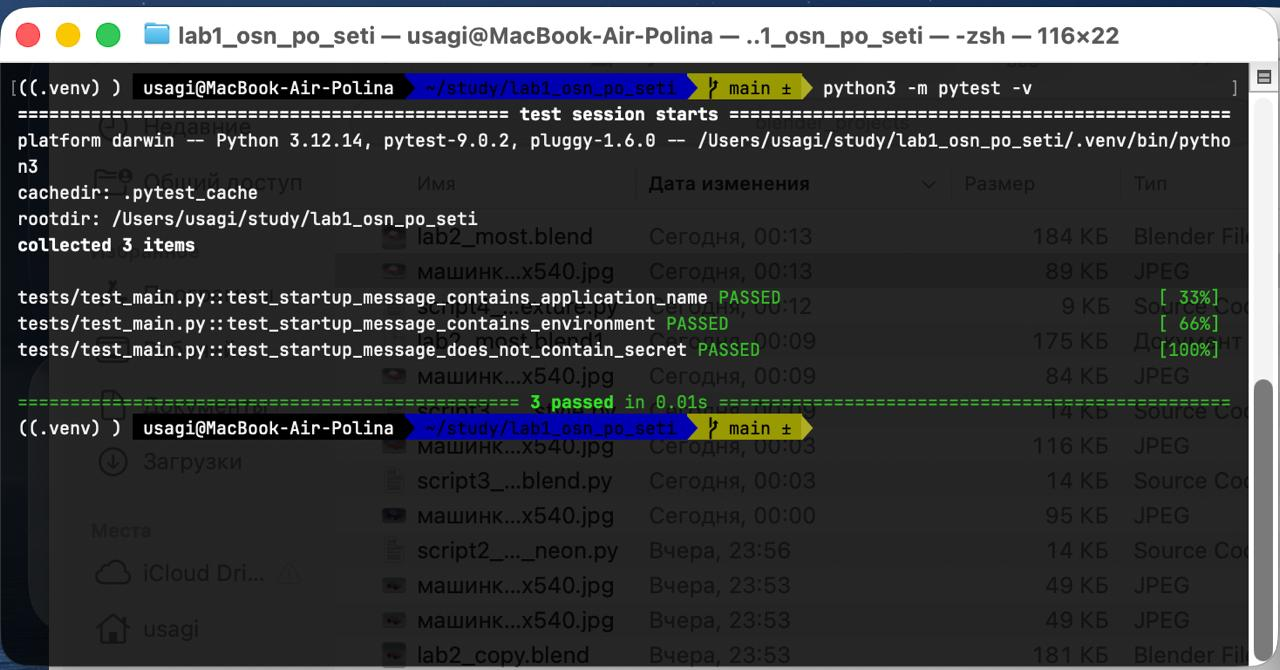
\includegraphics[width=0.9\textwidth]{03-tests.jpg}
\caption{Вывод трех существующих тестов прототипа.}
\end{figure}

\section{Таблица прослеживаемости}
\small
\begin{longtable}{p{2.8cm}p{1.5cm}p{1.5cm}p{1.5cm}p{2.8cm}p{2.0cm}}
\caption{Прослеживаемость AS $\rightarrow$ N $\rightarrow$ TH $\rightarrow$ RS $\rightarrow$ SEC $\rightarrow$ AT}\\
\toprule Актив & \shortstack{Наруши-\\тель} & Угроза & Риск & Требование & Проверка\\\midrule\endfirsthead
\toprule Актив & \shortstack{Наруши-\\тель} & Угроза & Риск & Требование & Проверка\\\midrule\endhead
AS-1, AS-2 & N-01 & TH-01 & RS-01 & SEC-1, SEC-14 & AT-10\\
AS-1, AS-5 & N-02 & TH-02 & RS-02 & SEC-1, SEC-14 & AT-11\\
AS-2, AS-5, AS-7 & N-03 & TH-03 & RS-03 & SEC-5, SEC-15 & AT-7\\
AS-4, AS-6 & N-03 & TH-04 & RS-04 & SEC-4, SEC-7 & AT-12\\
AS-5 & N-02 & TH-05 & RS-05 & SEC-6 & AT-13\\
AS-2 & N-02 & TH-06 & RS-06 & SEC-2, SEC-14 & AT-8\\
AS-2, AS-7 & N-04 & TH-07 & RS-07 & SEC-7, SEC-16 & AT-14\\
AS-5 & N-02 & TH-08 & RS-08 & SEC-2, SEC-3 & AT-9\\
AS-3 & N-05 & TH-09 & RS-09 & SEC-9, SEC-10 & AT-15\\
AS-10 & N-01 & TH-10 & RS-10 & SEC-18 & AT-16\\
AS-7, AS-10 & N-03, N-05 & TH-11 & RS-11 & SEC-7, SEC-16 & AT-17\\
AS-4, AS-5, AS-7 & N-05 & TH-12 & RS-12 & SEC-17 & AT-18\\
\bottomrule
\end{longtable}
\normalsize

\begin{figure}[H]\centering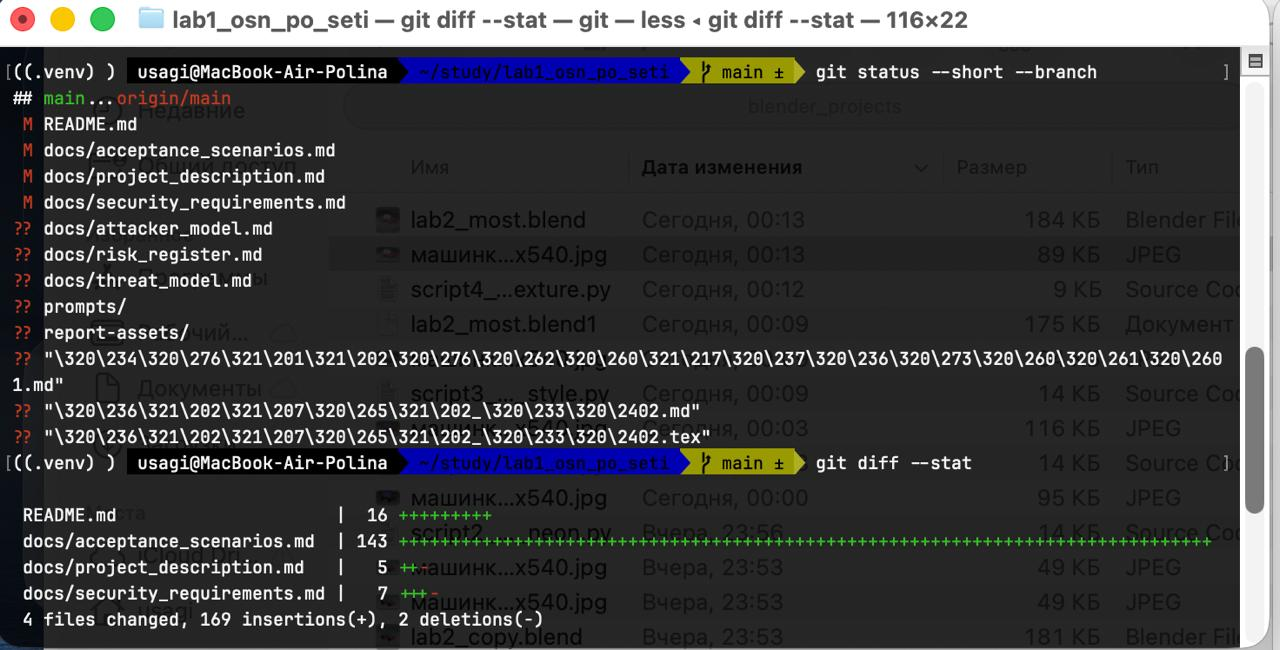
\includegraphics[width=0.9\textwidth]{04-working-tree.jpg}\caption{Статус и diff до фиксации результата.}\end{figure}
\begin{figure}[H]\centering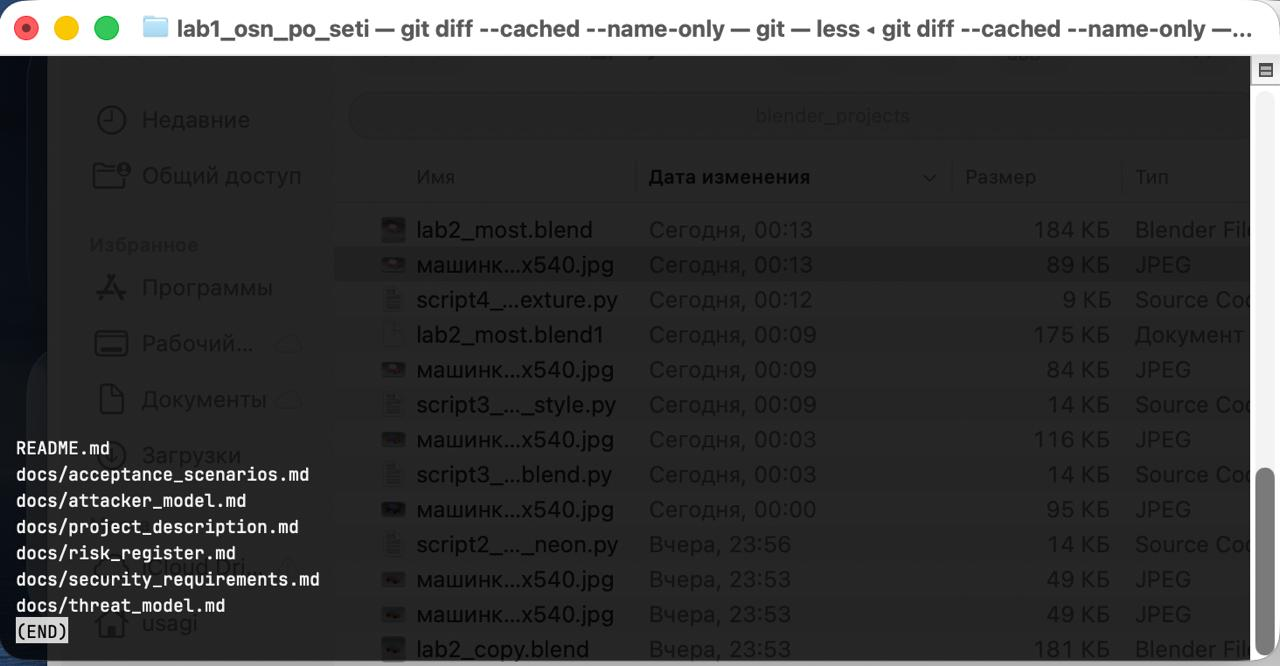
\includegraphics[width=0.9\textwidth]{05-staged-files.jpg}\caption{Подготовленный список файлов.}\end{figure}
\begin{figure}[H]\centering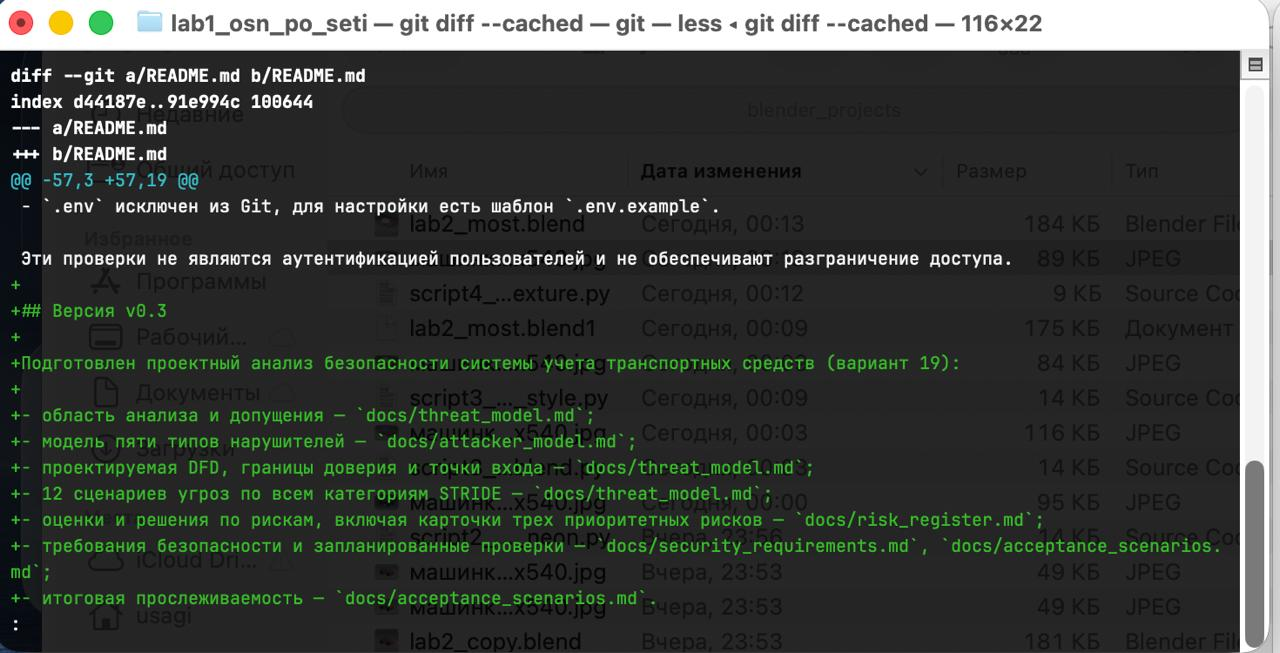
\includegraphics[width=0.9\textwidth]{06-readme-diff.jpg}\caption{Раздел v0.3 в README.}\end{figure}

\section{Проверка реализации и Git}
Команда \texttt{.venv/bin/python -m pytest -v} завершилась результатом \textbf{3 passed} на Python 3.12.14. Тесты проверяют только стартовое сообщение и отсутствие секрета в нем; учетные функции, роли и аудит ими не проверяются.

В истории имеется commit \texttt{9c9007e} с результатами ЛР №3 и аннотированный тег \texttt{v0.3}. На предоставленном снимке конечного состояния локальная ветка показана впереди \texttt{origin/main} на один commit; снимок сделан до отправки. Во время подготовки отчета commit \texttt{9c9007e} успешно отправлен в \texttt{origin/main} командой \texttt{git push origin main}. Тег v0.3 этой командой отдельно не отправлялся.
\begin{figure}[H]\centering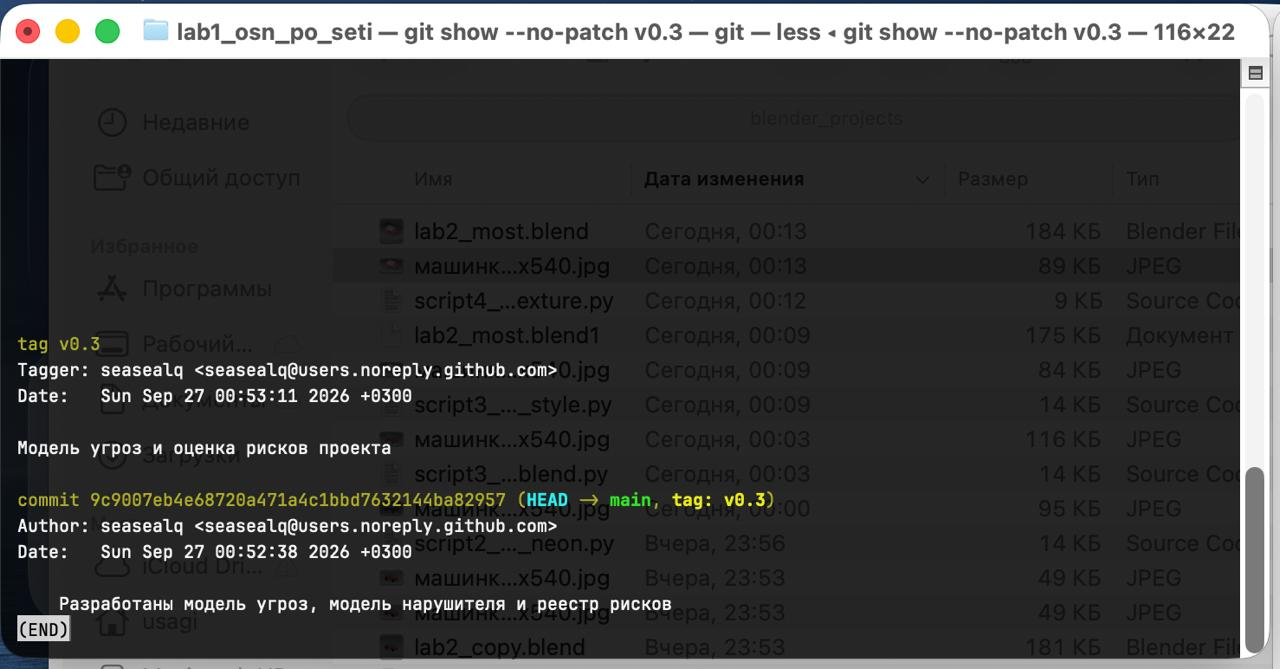
\includegraphics[width=0.94\textwidth]{07-v03-tag.jpg}\caption{Просмотр тега v0.3 и commit.}\end{figure}
\begin{figure}[H]\centering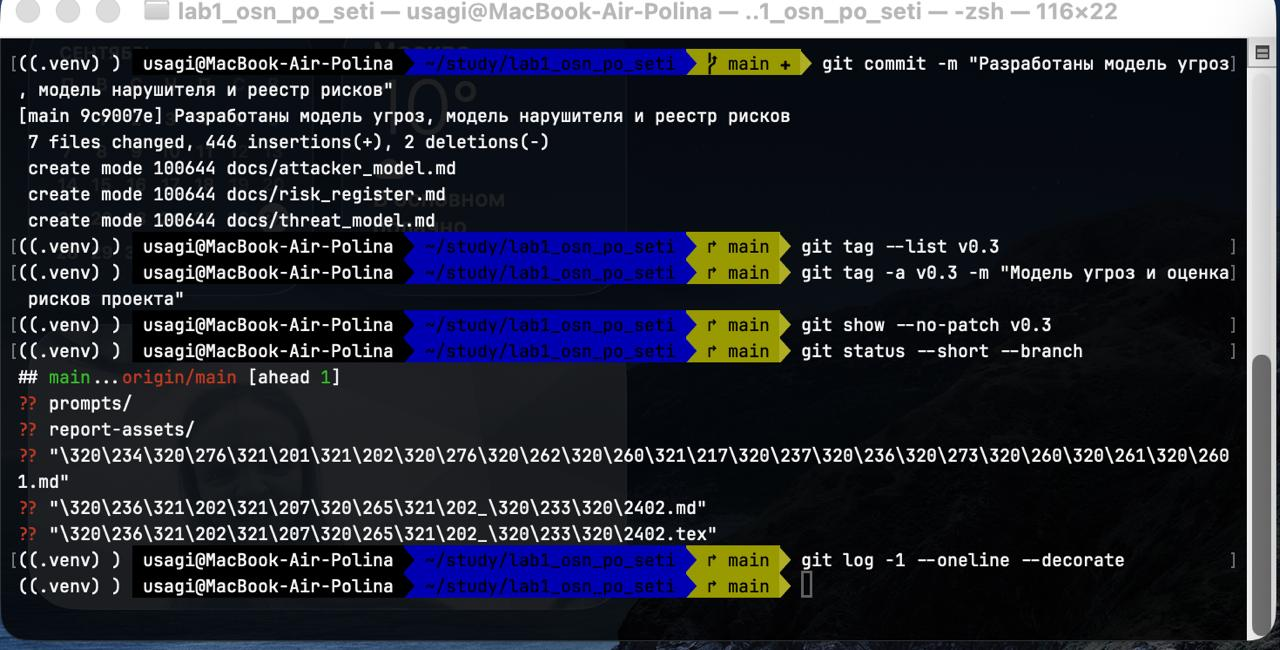
\includegraphics[width=0.9\textwidth]{08-commit-tag-status.jpg}\caption{Локальные commit, тег и статус до push.}\end{figure}

\section{Ответы на контрольные вопросы}
\begin{enumerate}[leftmargin=1.0cm]
\item \textbf{Чем угроза отличается от уязвимости?} Угроза — возможность нарушить защищаемое свойство; уязвимость — недостаток реализации, архитектуры, конфигурации или процесса, помогающий угрозе.
\item \textbf{Какие сведения нужны для сценария угрозы?} Нарушитель, исходный доступ, условие/недостаток, действие, затронутые элементы и активы, последствия и способы проверки мер.
\item \textbf{Почему зарегистрированный пользователь может быть нарушителем?} Он может использовать легитимный ограниченный доступ, чтобы попытаться выйти за свои полномочия, например запросить чужую поездку.
\item \textbf{Зачем указывать ограничения нарушителя?} Чтобы не приписывать ему несуществующие права и не завышать сценарий.
\item \textbf{Чем администратор приложения отличается от администратора ОС?} Первый управляет ролями внутри приложения, второй — ОС и процессами; полномочия не переходят автоматически.
\item \textbf{Какие элементы включает DFD?} Внешние сущности, процессы, хранилища, направленные потоки данных и границы доверия.
\item \textbf{Что обозначает граница доверия?} Переход между областями с разными полномочиями или условиями доверия, на котором нужны проверки.
\item \textbf{Почему граница может быть внутри одного сервера?} Процессы/учетные записи одного сервера могут иметь разные полномочия.
\item \textbf{Чем DFD отличается от схемы физической сети?} DFD показывает перемещение данных и логические компоненты; схема сети — узлы и соединения развертывания.
\item \textbf{Какие категории включает STRIDE?} Spoofing, Tampering, Repudiation, Information Disclosure, Denial of Service, Elevation of Privilege.
\item \textbf{Почему STRIDE не заменяет оценку риска?} Категория не задает вероятность и последствия сценария.
\item \textbf{Может ли сценарий иметь несколько категорий?} Да, если действие обоснованно затрагивает несколько свойств; в реестре указываются основная и дополнительная.
\item \textbf{Почему требование не доказывает устранение угрозы?} Требование описывает желаемое поведение; нужны реализация и проверка.
\item \textbf{Как связаны значимость актива и последствия?} Значимость — контекст ценности; S оценивается для конкретного сценария и не переносится автоматически из Ci/Ii/Ai.
\item \textbf{Ограничения формулы R=L×S?} Это грубая порядковая шкала, не процент и не стоимость; произведение не отражает всю неопределенность.
\item \textbf{Почему одинаковые баллы могут требовать разных решений?} Различаются активы, условия, последствия, восстановление и доступные меры.
\item \textbf{Какие способы обработки риска существуют?} Снизить, избежать, передать/разделить либо принять с контролем и пересмотром.
\item \textbf{Чем прогноз остаточного риска отличается от подтвержденного?} Прогноз предполагает будущую эффективность меры; подтверждение требует ее реализации и проверки.
\item \textbf{Как модель влияет на требования и тесты?} Сценарии выявляют нужные проверяемые требования, а тесты подтверждают их критерии и трассируются к угрозам.
\item \textbf{Когда пересматривать модель угроз?} При изменении функций, архитектуры, потоков, хранилищ, интерфейсов, ролей, развертывания, зависимостей или данных, а также после новых результатов проверок.
\end{enumerate}

\section{Вывод}
Для проектируемой системы учета транспорта определены участники, процессы, хранилища, потоки и границы доверия. На этой основе описаны возможности нарушителей и 12 сценариев STRIDE, связанные с учетными записями, карточками ТС, назначениями, поездками, отчетами и журналом. Для сценариев оценены вероятность и последствия по шкале методички, выбраны способы обработки, а требования связаны с проверками и таблицей прослеживаемости. Для трех приоритетных рисков определены меры и прогнозы остаточного риска. Функции и механизмы пока не реализованы, поэтому проверки остаются плановыми, а модель не доказывает безопасность работающей системы. Результаты служат основанием для дальнейшего проектирования защищенной архитектуры.

\clearpage
\renewcommand{\refname}{Список использованных источников}
\addcontentsline{toc}{section}{Список использованных источников}
\begin{thebibliography}{99}
\bibitem{method3} Методические указания «Лабораторная работа № 3. Разработка модели угроз и модели нарушителя программной системы».
\bibitem{owasp-threat} \mbox{OWASP} Foundation. Threat Modeling Cheat Sheet [Электронный ресурс]. URL: \url{https://cheatsheetseries.owasp.org/cheatsheets/Threat_Modeling_Cheat_Sheet.html} (дата обращения: 15.10.2026).
\bibitem{microsoft-stride} Microsoft. Microsoft Threat Modeling Tool threats: STRIDE model [Электронный ресурс]. Microsoft Learn. URL: \url{https://learn.microsoft.com/en-us/azure/security/develop/threat-modeling-tool-threats} (дата обращения: 15.10.2026).
\bibitem{nist-risk} Joint Task Force Transformation Initiative. Guide for Conducting Risk Assessments. NIST SP 800-30 Rev. 1. Gaithersburg: National Institute of Standards and Technology, 2012. URL: \url{https://csrc.nist.gov/pubs/sp/800/30/r1/final} (дата обращения: 15.10.2026).
\end{thebibliography}
\end{document}
